\documentclass[onecolumn,10pt]{asme2ej}
\usepackage[table]{xcolor}
\usepackage{epsfig} %% for loading postscript figures
\usepackage{amsmath}
\usepackage{graphicx}
\usepackage{mathtools}  
\mathtoolsset{showonlyrefs}  
\usepackage{amsbsy}
\usepackage{siunitx}
\usepackage[graphicx]{realboxes}
\usepackage[unicode]{hyperref}
\usepackage{rotating}
\usepackage{amsmath}
\usepackage{tabularx}
\usepackage{epsfig} 
\usepackage{booktabs}
\usepackage{multirow}
\renewcommand{\figurename}{Figure}
\usepackage[labelfont=bf]{caption}
\usepackage{adjustbox}
\usepackage{changepage}
\usepackage{titlesec}
\titleformat*{\section}{\Large\bfseries}
\titleformat*{\subsubsection}{\itshape}
\usepackage{geometry}
\geometry{a4paper,total={170mm,257mm},left=6cm,top=6cm}
\textwidth = 14 cm
\usepackage{fancyhdr}
\pagestyle{fancy}
%\fancyhead[RE,LO]{Essay 4 for module 7} % clear all header fields
\renewcommand{\headrulewidth}{0.4pt} % no line in header area
\fancyfoot{} % clear all footer fields
\fancyfoot[LE,RO]{\thepage}           % page number in "outer" position of footer line
%\renewcommand{\footrulewidth}{0.4pt}% default is 0pt
%\fancyfoot[RE,LO]{Word count: 1 483 words.} % other info in "inner" position of footer line

\usepackage{chngcntr}
\counterwithin{figure}{section}
\begin{document}


\begin{figure}[h]
	\includegraphics[width=0.05\textwidth]{figures/a}
	
	
	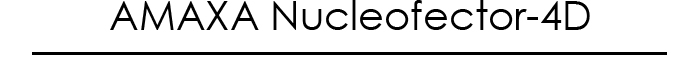
\includegraphics[width=0.33\textwidth]{figures/electro/Nucleo.jpg}
	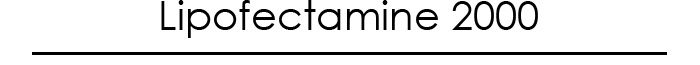
\includegraphics[width=0.33\textwidth]{figures/electro/Lipo2000.jpg}
	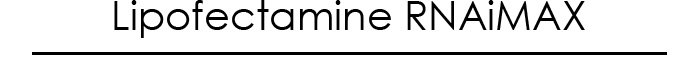
\includegraphics[width=0.33\textwidth]{figures/electro/LipoMAX.jpg}
	
	
	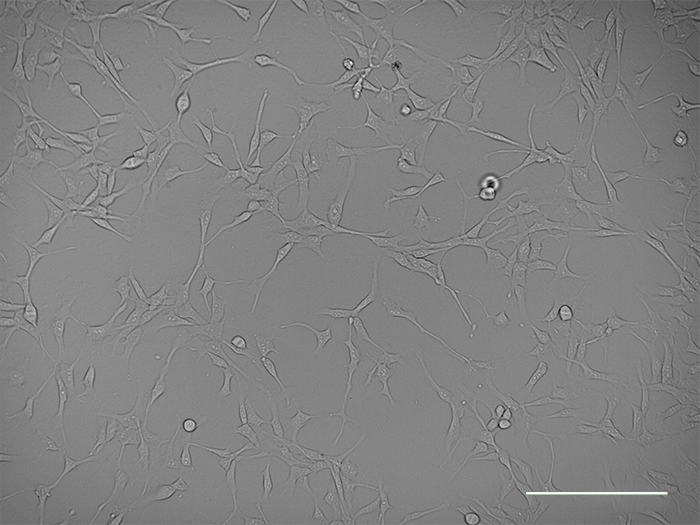
\includegraphics[width=0.33\textwidth]{figures/electro/ctrl-elec.jpg}
	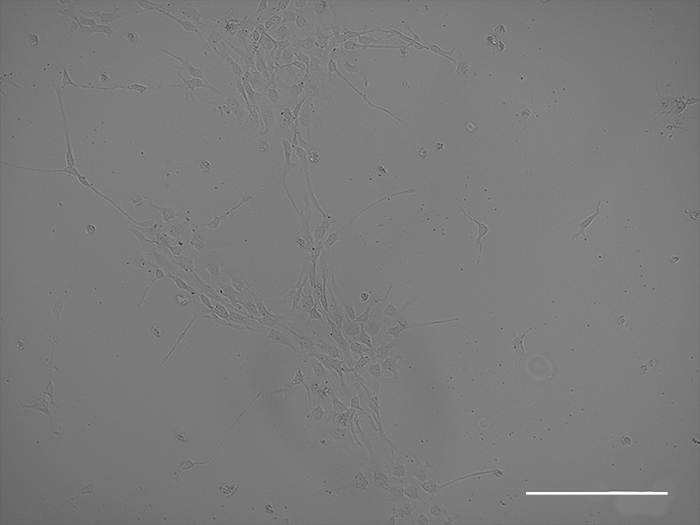
\includegraphics[width=0.33\textwidth]{figures/electro/BF2000(D1).jpg}
	\includegraphics[width=0.33\textwidth]{figures/electro/BFMAX(D3).jpg}
	
	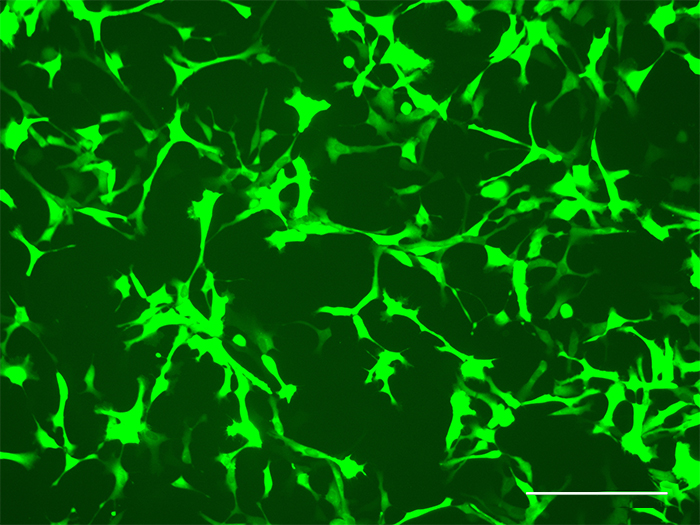
\includegraphics[width=0.33\textwidth]{figures/electro/ctrl-elec-g.jpg}
	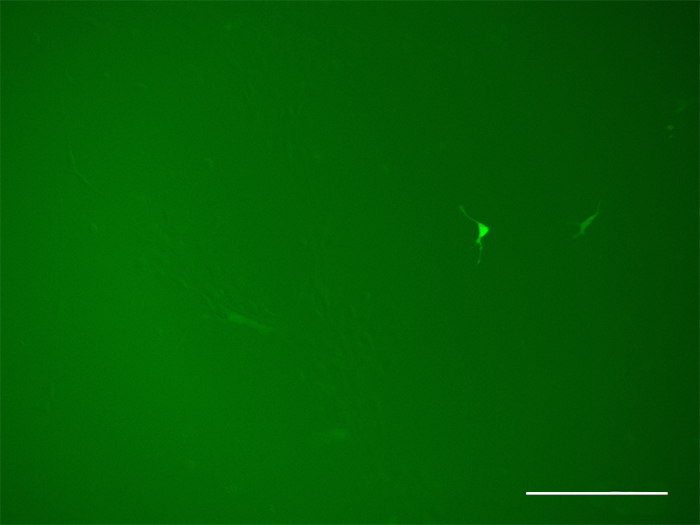
\includegraphics[width=0.33\textwidth]{figures/electro/G2000(D1).jpg}
	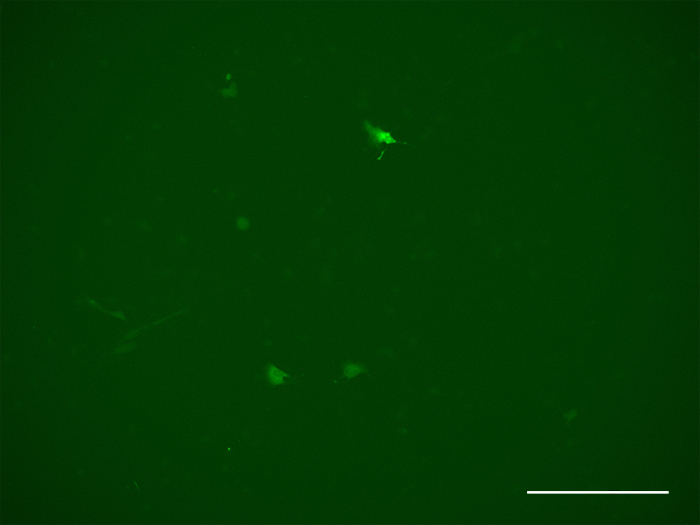
\includegraphics[width=0.33\textwidth]{figures/electro/GMAX(D3).jpg}
	
	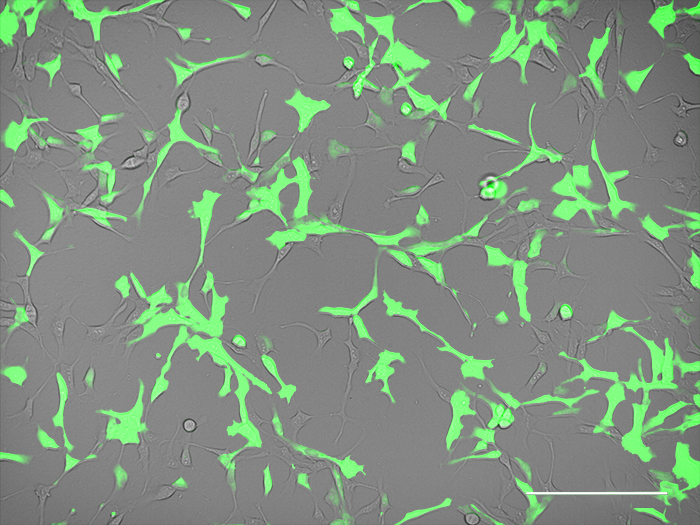
\includegraphics[width=0.33\textwidth]{figures/electro/ctrl-elec-m.jpg}
	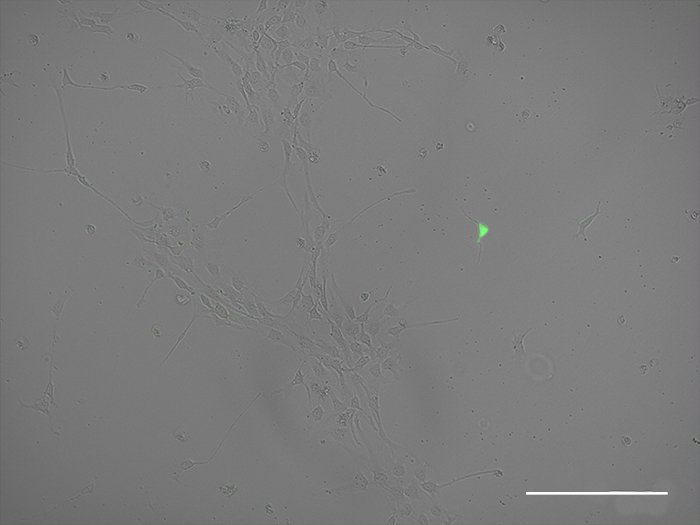
\includegraphics[width=0.33\textwidth]{figures/electro/Compo2000.jpg}
	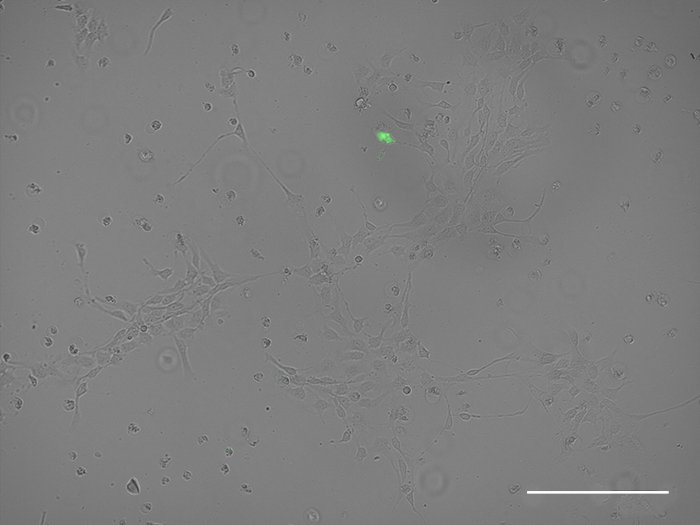
\includegraphics[width=0.33\textwidth]{figures/electro/CompoMAX.jpg}



\includegraphics[width=0.05\textwidth]{figures/b}


		\begin{center}
		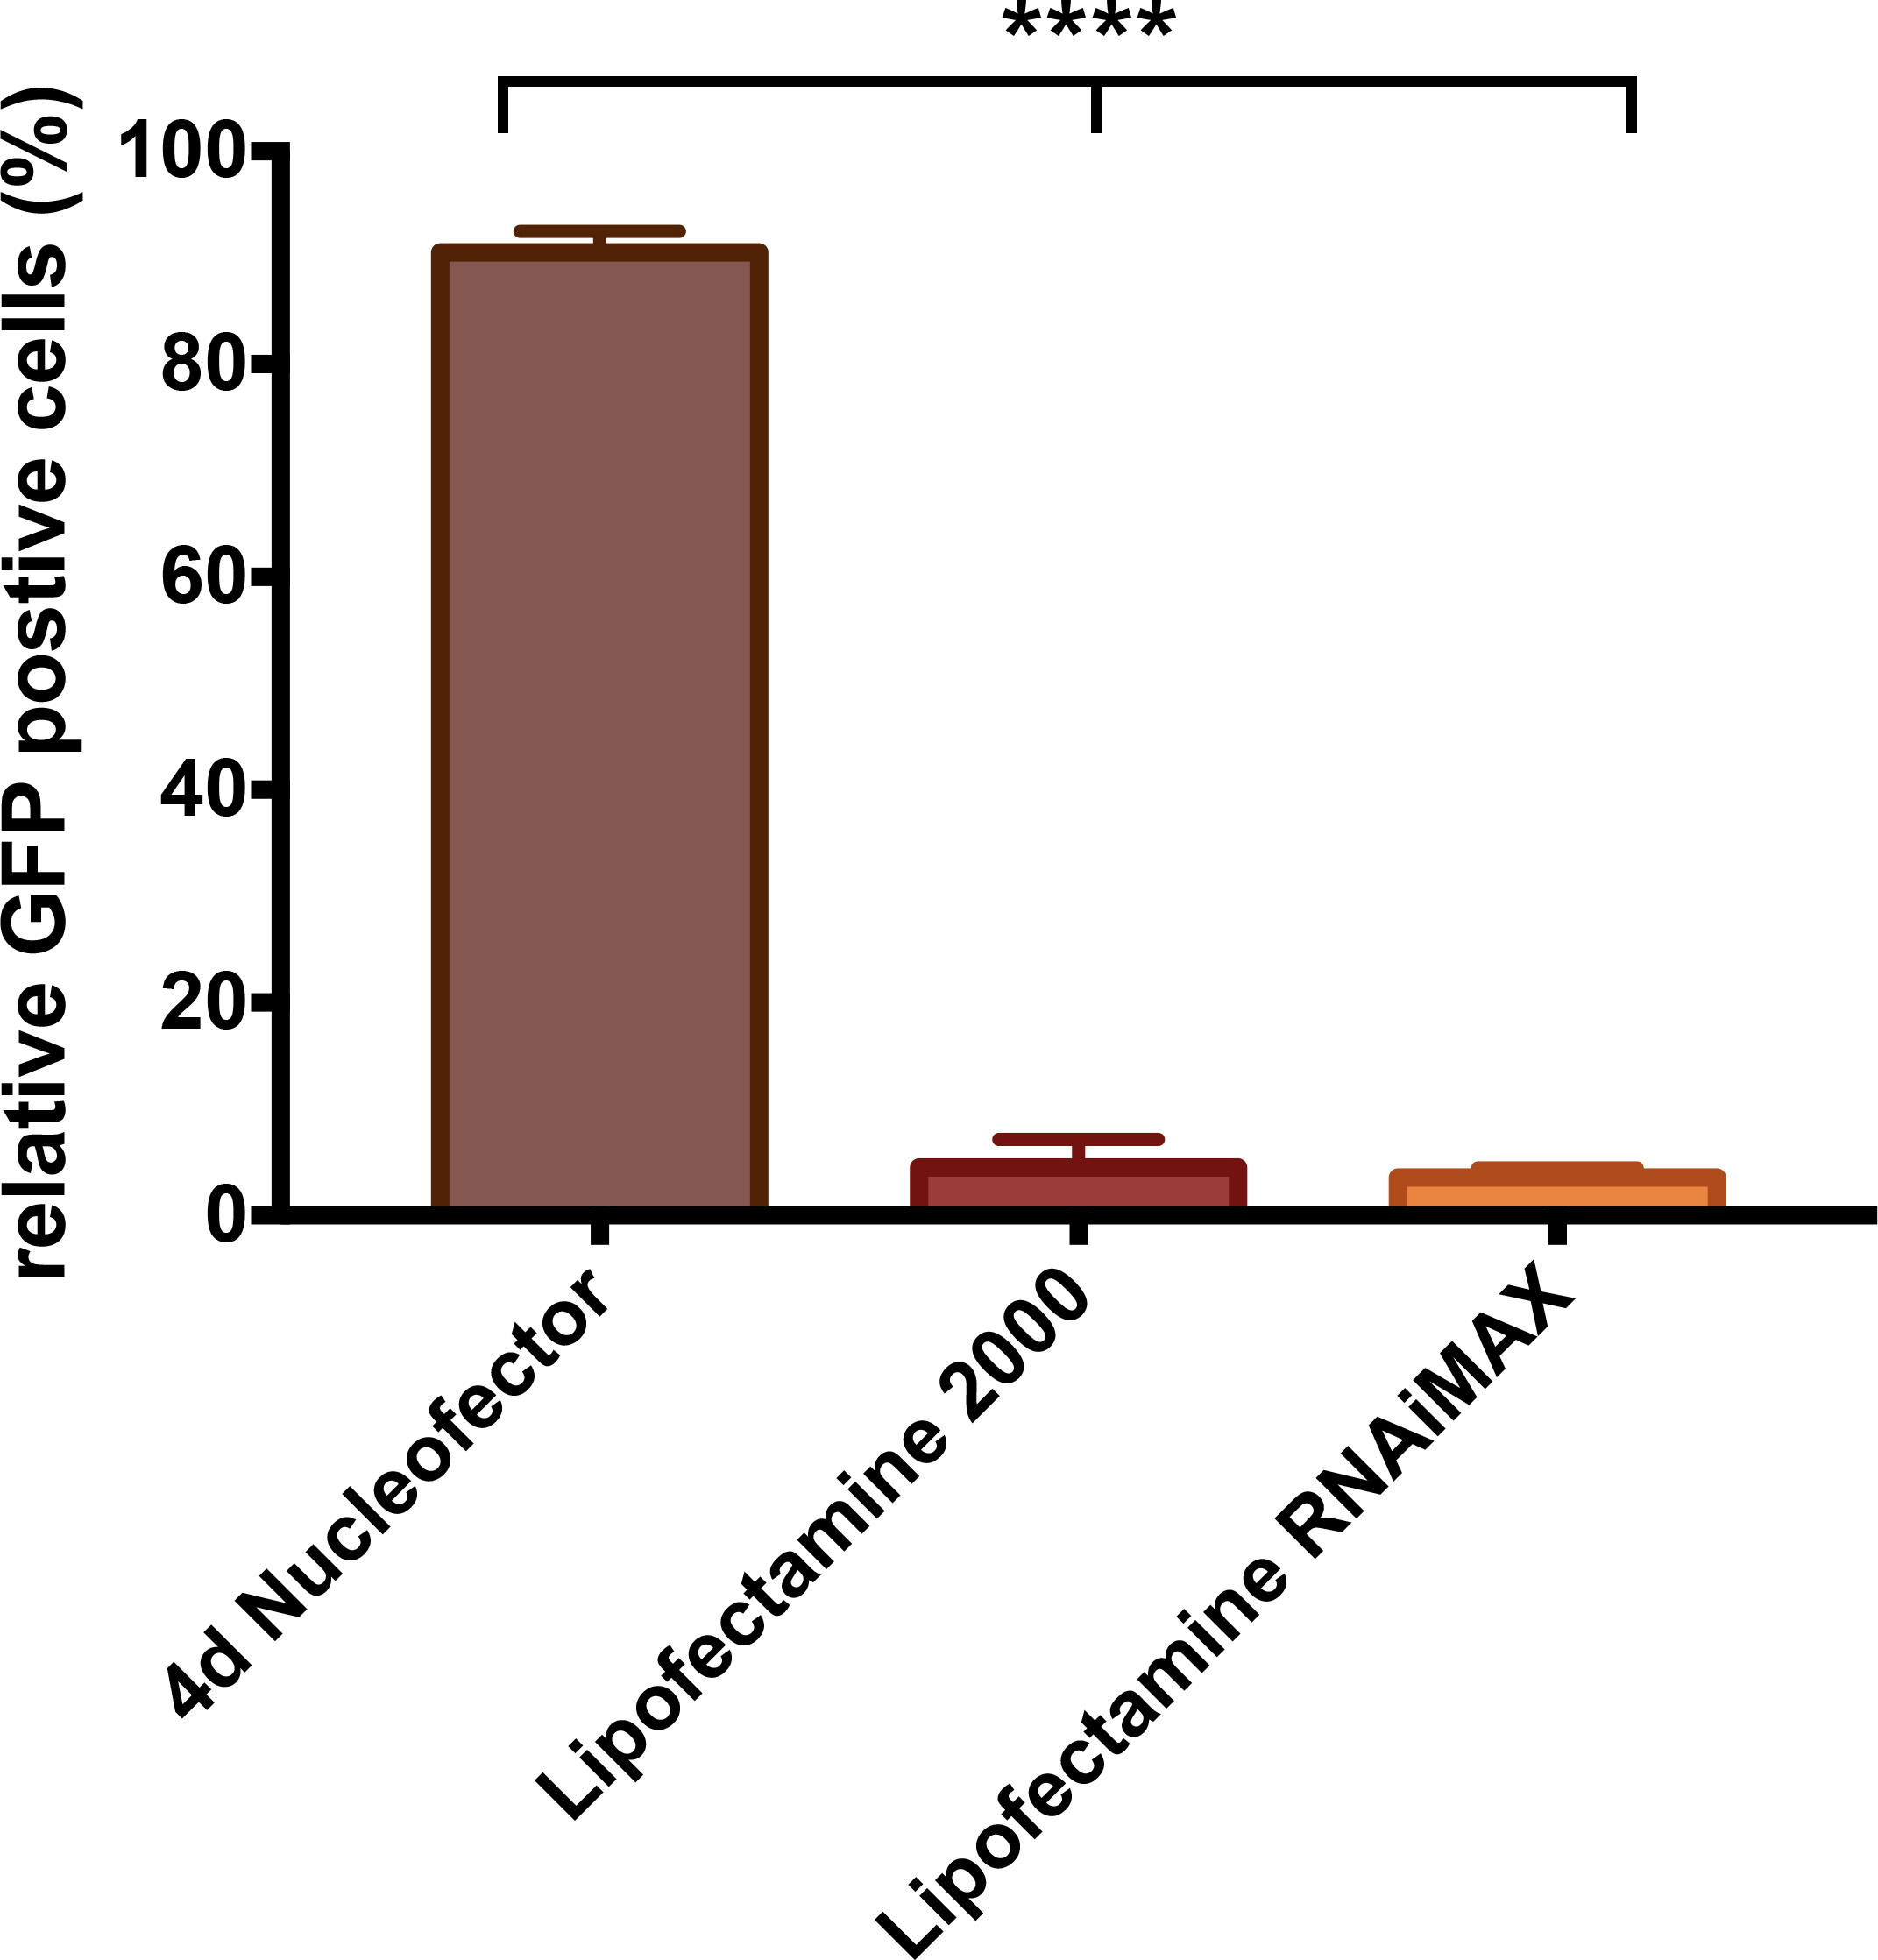
\includegraphics[width=0.5\textwidth]{figures/transfection.jpg}		
	\end{center}




\includegraphics[width=0.05\textwidth]{figures/c}


	\begin{center}
		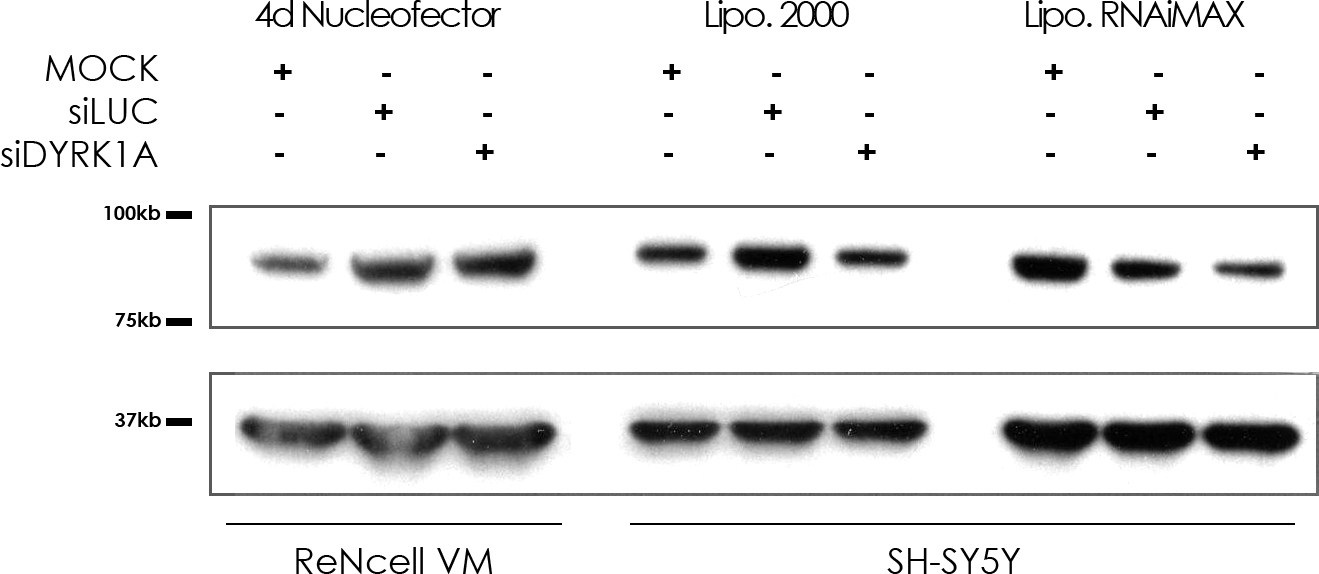
\includegraphics[width=0.8\textwidth]{figures/wb-sirna.jpg}	
	\end{center}
	
	\caption{\textbf{Transfection of Ren VM cells with DYRK1A siRNA.} Cells were transfected with DYRK1A siRNA by using the LONZA 4d Nucleofector protocol on primary cell lines. This was done with three different siRNA concentrations (100, 200 and 300 nM), with a mock (no DNA was added) and a negative control (luciferase). For n = 4, transfection efficiency is 33.75\% Unfortunately, the cells died before any quantifiable data was acquired - to be repeated. Might want to try with Lipofectamine considering electroporation is pricey (the cuvettes).
		Scale bar = 200 um.}
	\label{transfection}
\end{figure}


\end{document}

